\documentclass[tikz,border=8pt]{standalone}
\usepackage[T1]{fontenc}
\usepackage[utf8]{inputenc}
\usepackage{tikz}
\usetikzlibrary{arrows.meta,positioning,fit}

\begin{document}
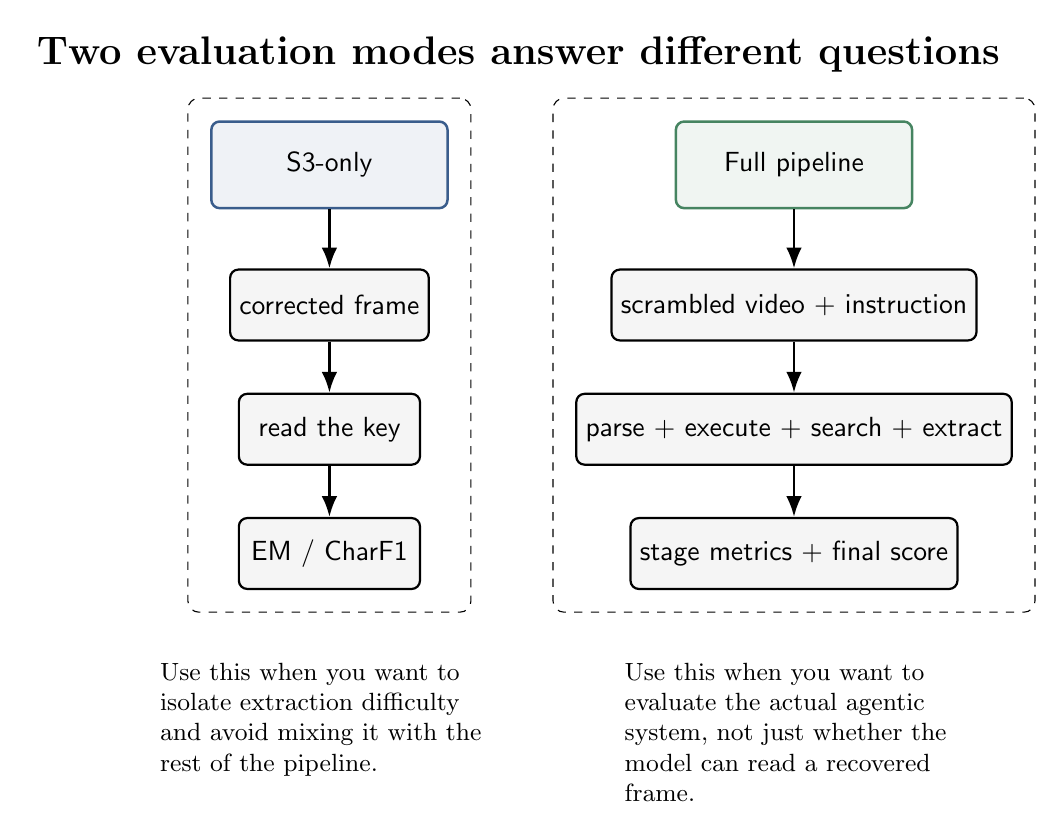
\begin{tikzpicture}[
  font=\sffamily,
  >=Latex,
  box/.style={draw, rounded corners=3pt, minimum width=3.0cm, minimum height=1.1cm, align=center, line width=0.9pt},
  small/.style={draw, rounded corners=3pt, minimum width=2.3cm, minimum height=0.9cm, align=center, fill=gray!8, line width=0.8pt},
  note/.style={font=\small, text width=4.3cm, align=left}
]

\definecolor{cblue}{RGB}{58,93,140}
\definecolor{cgreen}{RGB}{70,132,97}

\node[font=\bfseries\Large] at (4.7,3.0) {Two evaluation modes answer different questions};

% Left branch: S3-only
\node[box, draw=cblue, fill=cblue!8] (l1) at (2.3,1.6) {S3-only};
\node[small, below=0.75cm of l1] (l2) {corrected frame};
\node[small, below=0.65cm of l2] (l3) {read the key};
\node[small, below=0.65cm of l3] (l4) {EM / CharF1};
\draw[->, line width=1.0pt] (l1) -- (l2);
\draw[->, line width=1.0pt] (l2) -- (l3);
\draw[->, line width=1.0pt] (l3) -- (l4);
\node[note, below=0.8cm of l4] {Use this when you want to isolate extraction difficulty and avoid mixing it with the rest of the pipeline.};

% Right branch: full pipeline
\node[box, draw=cgreen, fill=cgreen!8] (r1) at (8.2,1.6) {Full pipeline};
\node[small, below=0.75cm of r1] (r2) {scrambled video + instruction};
\node[small, below=0.65cm of r2] (r3) {parse + execute + search + extract};
\node[small, below=0.65cm of r3] (r4) {stage metrics + final score};
\draw[->, line width=1.0pt] (r1) -- (r2);
\draw[->, line width=1.0pt] (r2) -- (r3);
\draw[->, line width=1.0pt] (r3) -- (r4);
\node[note, below=0.8cm of r4] {Use this when you want to evaluate the actual agentic system, not just whether the model can read a recovered frame.};

\node[draw, dashed, rounded corners=4pt, inner sep=8pt, fit=(l1)(l2)(l3)(l4)] {};
\node[draw, dashed, rounded corners=4pt, inner sep=8pt, fit=(r1)(r2)(r3)(r4)] {};

\end{tikzpicture}
\end{document}
